% main.tex -- draft v2 for IEEE QCE 2027 (full paper, ~8 pp. + refs)
% Compile: latexmk -pdf main.tex      (previous version: main_v1.tex)
%
% STATUS (2026-11-04): window w01, nights A and P5 analysed; night B interrupted (400 records)
% and not analysed. Offline re-analyses of w01 (research_notes/QEM combos and data reuse/,
% runs/nicdr_offline/, results_sim/nicdr/) are exploratory. Window w02vn (interleaved
% two-axis vnCDR) is pre-registered and runs tonight: every \TBD{...} in Sec. IV-H is a
% placeholder for its result.
% Number sources: runs/odra_campaign/w01{A,P5}/*.csv, results/depth_regression_w01P5.csv,
% figs/fig_numbers.txt, figs/p5_robust_numbers.txt (figs/p5_robust_paper.py),
% research_notes/QEM combos and data reuse/prototypes/out/*, runs/nicdr_offline/*,
% results_sim/nicdr/*, review/{recenzja,weryfikacja}.md, preregistration_w02_vncdr.md.

\documentclass[conference]{IEEEtran}
\IEEEoverridecommandlockouts
\usepackage[T1]{fontenc}
\usepackage[utf8]{inputenc}
\usepackage{amsmath,amssymb,mathtools}
\usepackage{booktabs}
\usepackage{array}
\newcolumntype{L}[1]{>{\raggedright\arraybackslash}p{#1}}
\usepackage{graphicx}
\usepackage{xcolor}
\usepackage{url}
\usepackage[hidelinks]{hyperref}
\usepackage{cite}

\newcommand{\TBD}[1]{\textcolor{red}{\textbf{[TBD: #1]}}}
\newcommand{\ev}[1]{\langle #1\rangle}
\newcommand{\ket}[1]{|#1\rangle}
\newcommand{\Oid}{O_{\mathrm{id}}}
\newcommand{\CZ}{\mathrm{CZ}}
\newcommand{\PRX}{\mathrm{PRX}}
\newcommand{\Var}{\operatorname{Var}}
\newcommand{\E}{\mathbb{E}}
\newcommand{\arm}[1]{\texttt{#1}}
\newcommand{\expl}{\textsuperscript{\textit{e}}}

\begin{document}

\title{Honest Hardware Evaluation of Quantum Error Mitigation: Equal-Budget Controls,
Pre-Registration and a Catalogue of Pitfalls on a Five-Qubit Star Processor}

\author{\IEEEauthorblockN{Karina Le\'skiewicz}
\IEEEauthorblockA{KN Axion, Wroc{\l}aw University of Science and Technology
(Politechnika Wroc{\l}awska), Poland}}

\maketitle

% ---------------------------------------------------------------------------------------
\begin{abstract}
Hardware comparisons of quantum error mitigation (QEM) routinely mix unequal shot budgets,
uncontrolled drift and post-hoc analysis choices. We present a protocol for honest hardware
evaluation of QEM---equal-shot-budget controls, matched-cost negative controls,
pre-registered analysis and full per-circuit provenance---and apply it to zero-noise
extrapolation (ZNE), Clifford data regression (CDR) and Pauli twirling on the five-qubit
star-topology IQM ODRA~5 processor. The protocol turns most apparent effects into pitfalls,
which we catalogue with hardware evidence: at equal cost CDR's 42-fold budget advantage over
ZNE shrinks: CDR's error saturates at 4--8 times ZNE's budget, at ZNE's budget it ties
readout-corrected ZNE at 12~CZ (ZNE error $0.045\to0.016$ with readout correction), and at
39~CZ it has no clear per-point advantage over ZNE. At 39~CZ ZNE has collapsed onto the
noise floor, which a garbage-folding control and a floor-referenced SNR detect but negative
mass and a zero-referenced SNR do not; an identity-folding control, valid in simulation, is
invalid on hardware because of $T_1$; and an apparent twirling penalty at 12~CZ is an artefact
of the log-error floor, while twirling consistently raises the CDR fit's $r^2$ and its gain is
limited by frame-to-frame variance (12--29 times the shot variance). An identity-insertion
experiment decomposes the noise axis: at fixed gate count each microsecond raises the raw
error $1.43$-fold (robust to small-cluster inference), whereas the CZ effect at fixed
duration is unresolved, and the error left after CDR grows with CZ count. Only the duration
effect is a confirmed pre-registered result; the other findings are exploratory and are
labelled so. A new pre-registered test of interleaved two-axis variable-noise CDR is
\TBD{w02vn primary result in one sentence}.
\end{abstract}

\begin{IEEEkeywords}
quantum error mitigation, zero-noise extrapolation, Clifford data regression, Pauli
twirling, benchmarking methodology, pre-registration, superconducting qubits
\end{IEEEkeywords}

% ---------------------------------------------------------------------------------------
\section{Introduction}

Quantum error mitigation (QEM) trades variance for bias: a classical post-processing of
many, possibly modified, circuit executions reduces the bias that hardware noise introduces
into an expectation value $\ev{O}$, at the price of a sampling overhead that grows
exponentially with the noise~\cite{temme2017,li2017,cai2023,takagi2022,quek2024}. Whether a
method ``works'' on a given device is therefore a quantitative question about cost and
error, and answering it on hardware is harder than it looks. Methods are compared at
whatever budget each happens to use; a twirled estimator averaged over $M$ frames is set
against a baseline measured once; drift between blocks run hours apart is attributed to
the method; and analysis choices---a log transform, a floor, a diagnostic threshold---are
made after the data are seen. K\"oster and Mauerer recently showed on IQM hardware that ZNE
can report ``improvements'' that a matched-cost garbage-folding control reproduces or
exceeds~\cite{koster2026}.

This paper is about such failure modes. We evaluate ZNE~\cite{temme2017,giurgica2020}, CDR
\cite{czarnik2021} and Pauli twirling~\cite{wallman2016,hashim2021} on the five-qubit
star-coupled IQM ODRA~5, with one frozen variational classifier compiled to 12 and 39 CZ
gates and a pre-analysis plan frozen before any error was computed. The design was built to
detect artefacts, and it did: most effects that a conventional analysis would report turned
out, under the controls, to be budget, readout, floor, frame-count or block-time effects.
Our contributions are:
\begin{itemize}
  \item \textbf{A protocol for honest hardware evaluation of QEM}: equal-shot-budget arms
  inside CDR (an \arm{off\_copies} control isolates twirling from averaging), an offline
  equal-budget re-analysis across methods from archived counts, matched-cost negative
  controls for ZNE, pre-registration with reported deviations, and per-circuit provenance
  (counts, frames, seeds, calibration IDs) from which every number is recomputed.
  \item \textbf{A catalogue of pitfalls confirmed on hardware} (Table~\ref{tab:pitfalls}),
  among them: the CDR--ZNE ranking changes at equal cost and after readout correction; ZNE
  collapse is invisible to negative-mass and zero-referenced SNR diagnostics; an identity-folding
  control fails through $T_1$; geometric error ratios are driven by the log floor; native
  twirling is limited by the number of frames; and block-time and calibration confounds make
  cluster-robust $p$-values with 8 clusters anti-conservative.
  \item \textbf{A noise-axis decomposition}: identity insertion (CZ$\cdot$CZ pairs vs.\
  duration-matched idling) separates CZ count from duration; raw error follows duration,
  the residual after CDR follows CZ count.
  \item \textbf{Negative results} for noise-model-informed CDR, CDR--ZNE hybrids and duration
  covariates (Table~\ref{tab:neg}), and the pre-registered design of a new interleaved
  two-axis variable-noise CDR (vnCDR) test, whose result is reported in
  Section~\ref{sec:w02vn}.
\end{itemize}

\emph{Related work.} Matched-cost garbage folding and the collapse of Richardson
extrapolation into a rescaling of one measurement are due to~\cite{koster2026}; our ZNE
results are a replication on another IQM device with a sharper control (identical CZ
skeleton and PRX count) and with diagnostics that fail. Finite-shot help--harm boundaries of
ZNE were analysed in~\cite{krebsbach2022,scavino2026}. vnCDR~\cite{lowe2021} and UNITED
\cite{bultrini2023} combine noise scaling with Clifford training; they were evaluated in
simulation, and UNITED showed that the best method depends on the total budget and that
learning-based methods become fragile to shot noise at high noise. Learning-based PEC from
Clifford variants~\cite{strikis2021}, sparse Pauli--Lindblad noise learning
\cite{vandenberg2023,kim2023} and verifiable benchmark circuits that correct ZNE
\cite{harris2026} are the closest noise-informed approaches; frugal CDR~\cite{czarnik2022}
reduces CDR's cost. To our knowledge, no hardware study has compared CDR with and without
twirling at a controlled equal budget, but our literature search was not exhaustive.

% ---------------------------------------------------------------------------------------
\section{Background}\label{sec:background}

\emph{Noise as compression.} A mitigation method measures circuits $C_1,\dots,C_K$ and
returns $\hat O=g(E_1,\dots,E_K)$; its quality is $\mathrm{MSE}=B^2+\Var\hat O$. Under
\emph{global} depolarization amplified $\lambda$-fold,
\begin{equation}
  E(\lambda)\approx f+(\Oid-f)\,e^{-\gamma\lambda},
  \label{eq:compress}
\end{equation}
with floor $f$, the value of $\ev{O}$ under full decoherence. For the mean-$Z$ observable used
here, $f=0$ for pure depolarization, but $T_1$ relaxation towards $\ket0$ and asymmetric
readout make $f>0$ on transmons, so $f$ must be measured. Local, correlated and coherent
noise break~\eqref{eq:compress}; this is where both methods' limits come from.

\emph{ZNE and its collapse.} Global folding $U\to U(U^\dagger U)^k$ gives $\lambda=2k+1$;
Richardson extrapolation at $\lambda\in\{1,3,5\}$ is $\hat E=\sum_kc_kE(\lambda_k)$ with
$c=(\tfrac{15}{8},-\tfrac54,\tfrac38)$. Since $\sum_kc_k=1$, any \emph{$\lambda$-independent
offset passes through unchanged}---a constant readout bias is not mitigated. With $S$ shots
split over $|\Lambda|$ scales, ZNE lowers the MSE only above
$S^\ast=\kappa V/(B^2-B_{\text{ZNE}}^2)$, with $\kappa=|\Lambda|\sum_kc_k^2-1=14.66$ for
$\{1,3,5\}$ (11.25 under Neyman allocation $n_k\propto|c_k|\sigma_k$)~\cite{krebsbach2022}.
When the circuit is so deep that $E(3)\approx E(5)\approx f$, $\hat E=\tfrac{15}{8}E_1-\tfrac78f$
is a rescaled single measurement that can mimic mitigation~\cite{koster2026}. We use four
diagnostics: (i) a \emph{garbage-folding} control $U(V^\dagger U)^k$, with $V$ of identical CZ
skeleton and PRX count but random angles (same cost, function destroyed); (ii) the
floor-tracking distance $|\hat E-(c_1E_1+(1-c_1)f)|$; (iii) the SNR of the largest scale
\emph{against the floor}, $|E(\lambda_{\max})-f|/\mathrm{SE}$; and, as pre-registered, (iv) the
negative mass $W_{\text{neg}}$ of Richardson applied to the $2^5$ outcome probabilities and
the SNR against zero. (iv) is blind to collapse by construction: when $P(\lambda_{3,5})$ are
near uniform $u$, $\hat P=\tfrac{15}{8}P_1-\tfrac78u$ is negative only where $P_1<0.47u$, and
$|E(\lambda_{\max})|/\mathrm{SE}$ measures the distance of the floor from zero.

\emph{CDR.} CDR~\cite{czarnik2021,lowe2021} measures Clifford versions of the target, whose
ideal values a stabilizer simulator gives~\cite{gottesman1998,aaronson2004}, and fits
$\Oid\approx aE+b$. Under global depolarization the map is affine and shared, and its
intercept absorbs readout offsets; circuit-dependent (local, coherent) noise scatters the
training points and lowers $r^2$. Shot noise in the regressor attenuates the OLS slope; an
errors-in-variables fit~\cite{fuller1987} corrects it but is unstable at small spread. vnCDR
\cite{lowe2021} measures every training circuit at several noise levels $E^{(\ell)}$ and fits
$\Oid\approx\sum_\ell a_\ell E^{(\ell)}$ (we add an intercept $b$), a Richardson-like
combination whose weights are learned from Clifford data.

\emph{Pauli twirling.} Wrapping each CZ in a random Pauli frame $(A,\CZ A\CZ^\dagger)$ leaves
the circuit unchanged; averaged over \emph{all} frames, the gate error becomes a Pauli channel
with the same Pauli error rates and no coherent off-diagonal part~\cite{wallman2016,hashim2021}.
This motivates twirling as a precondition for CDR's single affine map. With $M$ sampled frames
the average holds only in expectation, and each frame is a separate circuit, which multiplies
the cost by $M$ and is why equal-budget controls are needed.

% ---------------------------------------------------------------------------------------
\section{Methods}\label{sec:methods}

\subsection{Device, compilation and workload}
IQM ODRA~5 has five transmons in a star (hub QB3), native $\PRX(\theta,\varphi)$ and CZ (hub
edges only), virtual $Z$. A calibration dump of 2026-08-03 gave CZ errors of 0.78--1.05\% and
PRX errors of 0.10--0.12\%. All circuits go through one deterministic path: Qiskit
\cite{qiskit2024} 2.4.1, basis $\{\texttt{r},\texttt{cz}\}$, identity layout, optimization
level~1, \texttt{seed\_transpiler}=42, then our single-qubit merging pass, which fuses every
run of single-qubit gates between two CZs into at most one PRX (pushing $R_Z$ through CZ) and
never touches the CZ skeleton. Two pitfalls motivated this. An unseeded path gave five
distinct CZ skeletons in five compilations, and separately compiled CDR training circuits
matched their target's routing in only 0--2 of 10 cases; we therefore build training circuits
on the target's native circuit (100\% skeleton match in the data). And unmerged twirl frames
lengthen the circuit (12~CZ: from 40 to 92 single-qubit gates); after merging, applied to all
arms, targets carry 20 vs.\ 23--27 PRX (untwirled vs.\ twirled) at 12~CZ and 80 vs.\ 80--83 at
39~CZ.

The workload is a frozen data-re-uploading classifier~\cite{perezsalinas2020,schuld2021} on
the \emph{two curves} dataset~\cite{bowles2024}: five qubits, three layers, 55 weights, output
$\ev{\bar Z}$ with $\bar Z=\frac15\sum_qZ_q$. Star-entangled and circular-entangled versions,
trained separately and frozen, compile to \textbf{12 and 39 CZ} on the star (routing through
the hub). They are different functions, so the ``ladder'' is a ladder of workloads, not a
pure manipulation of CZ count. Eight evaluation points per rung are drawn deterministically,
two per quartile of the star model's ideal margin. The primary metric is the per-point error
$\varepsilon=|\hat O-\Oid|$.

\subsection{CDR arms at equal budget}
Every CDR arm uses $n_{\text{train}}=20$ training circuits, $M=6$ and $S=8192$:
$B_{\text{CDR}}=(n_{\text{train}}+1)MS=1{,}032{,}192$ shots per point, verified in the data.
The target is always measured $M$ times; arms differ in how the training half is spent: $M$
identical copies (\arm{off\_copies}, control), $M$ native frames after routing, merged
(\arm{twirl\_native}), $M$ logical frames before routing (\arm{twirl\_logical}; SWAP-derived
CZs stay bare), or $n_{\text{train}}M=120$ distinct circuits with one frame each
(\arm{spread}). Training circuits come from a \arm{near\_target} sampler seeded per point; the
logical-vs-native comparison uses a legacy \arm{shared\_random} set whose training circuits
are identical for all points. Despite the name, the code snaps \emph{all} rotations to Clifford
angles and drops $\theta=0$ rotations, so training circuits are Clifford, carry about half the
target's PRX (10 vs.\ 20 at 12~CZ) and are 0.08--0.20\,\textmu s shorter; at 39~CZ 78--85\% of them
have ideal value exactly~0.

\subsection{ZNE, controls and readout correction}
ZNE folds the compiled native circuit (never re-transpiled, barriers between folds),
$S=8192$ per scale, $B_{\text{ZNE}}=24{,}576$ shots per point, Richardson without clamping.
The genuine, garbage and identity variants share the $\lambda=1$ measurement and have identical
CZ skeletons and PRX counts at each scale. The garbage twin $V$ is drawn separately for
$\lambda=3$ and $5$. Identity folding replaces $U^\dagger U$ by a block with the same CZ
sequence in which each single-qubit gate is paired with its inverse. The pre-registered floor
$f$ is the garbage value at $\lambda=5$ of the same point; we also use the mean garbage floor.
\emph{Readout correction (REM, offline).} For mean-$Z$, per-qubit inversion
$Z=(Z_m-(e_{10}-e_{01}))/(1-e_{01}-e_{10})$ with the vendor's single-shot readout errors of the
night's calibration set ($e_{01}=0.3$--$0.8\%$, $e_{10}=2.5$--$5.1\%$) is exact, because
$\bar Z$ depends only on single-qubit marginals; the implied offset is $+0.029$, the gain
0.96. REM costs no shots.

\subsection{Equal-budget accounting across methods (offline)}
Within CDR, budgets are equal by design. Across methods they are not ($B_{\text{CDR}}\approx
42B_{\text{ZNE}}$), so we re-analyse CDR at smaller budgets from the archived counts. Because
$\bar Z$ depends only on the Hamming weight, subsampling a circuit's counts is exact
multivariate-hypergeometric sampling over six categories. At a budget $B$, the target gets
$T=\min(49{,}152,B/3)$ shots and each of the 20 training circuits $(B-T)/20$; the reported
error is the expectation over 200 draws per point (600 for the pre-specified ZNE-budget
allocation $8192+20\times819$). ZNE cannot be re-analysed upwards: its error is a single
realization (SE $\approx0.011$ per point). Subsamples inherit the drift of their block.

\subsection{Identity insertion (night P5)}
On the 12-CZ star circuit we insert $k\in\{6,12,20\}$ identity pairs at evenly spread CZ
positions: \emph{cz\_pairs} inserts $\CZ\cdot\CZ$ on an existing edge (24, 36, 52~CZ; same PRX
and function), \emph{idle\_matched} inserts a delay of two CZ durations (12~CZ, same scheduled
duration). Training circuits receive identical insertions. Durations are computed ASAP
schedules ($t_{\text{CZ}}=60$\,ns, $t_{\text{PRX}}=20$\,ns; IQM rounds delays up), from 0.80 to
3.20\,\textmu s; they are not measured. We fit
$\log\varepsilon_{ij}=\alpha_i+\beta_{\text{CZ}}n_{\text{CZ},j}/10+\beta_t t_j+u_{ij}$
with point fixed effects, 56 observations, \arm{off\_copies} only. With $G=8$ clusters the
pre-registered cluster-robust normal reference is anti-conservative; we report the $t(G-1)$
reference and an exact restricted wild-cluster bootstrap~\cite{cameron2008} (all $2^8$
Rademacher sign vectors; smallest attainable $p=2/256$). The $L=6,9,13$ classifiers in the same
night are different functions and are not used.

\subsection{Nights, blocking and calibration}
Night A (12 and 39~CZ, all CDR arms and ZNE variants, 10,192 circuits, 2026-10-24, one
calibration set) and night P5 (10 rungs, 10,080 circuits, 2026-10-24/25) form window
\texttt{w01}; night B (30 and 57~CZ) was interrupted after 400 records when the device stopped
responding and is not analysed. A block is one (rung, arm) unit; block order is randomized
with the window seed. Each condition is a single block, so arms of a rung are hours apart.
The calibration-set ID is read before and after every block and every record carries the
start-of-block ID: a recalibration is detected per block, drift between recalibrations is
not. In P5 the calibration changed during \texttt{star\_cz52}; \texttt{star\_cz24} ran
entirely on the new set ($T_1$ of QB1 15.6$\to$20.8\,\textmu s, QB2 12.7$\to$17.0\,\textmu s), and
all idle blocks and the base ran 21:01--02:36~UTC, all CZ-pair blocks 04:21--09:21~UTC.

\subsection{Statistics and pre-registration of \texttt{w01}}
The plan and its analysis code were committed and tagged (\texttt{prereg-v1}) before any error
of \texttt{w01} was computed~\cite{nosek2018}, but after night A had started: it is a
pre-analysis plan, not a pre-data registration, and hypotheses were informed by pilot windows.
The primary family was H1 (\arm{twirl\_native} below \arm{off\_copies}, 32 pairs over nights A+B),
H3 (native $\le$ logical), H6 (\arm{spread} below \arm{twirl\_native}), H7a (more CZ at fixed
duration raises raw error) and H7b (longer duration at fixed gates raises raw error): Wilcoxon
signed-rank tests~\cite{wilcoxon1945} on $\log\varepsilon$ (floor $10^{-4}$), Holm correction
\cite{holm1979}. H4 (ZNE pays: below raw and garbage, median $W_{\text{neg}}\le0.02$, median
SNR $\ge2$) was secondary. Everything else in this paper---REM, equal-budget curves, $r^2$,
frame variance, floor sensitivity, robust P5 inference, hybrids---is exploratory: many variants
were tried on 8 points per rung, and $p$-values outside the family are uncorrected (two-sided
Wilcoxon unless stated; marked\,\expl).

\subsection{Window \texttt{w02vn}: interleaved vnCDR (pre-registered)}
\label{sec:w02vn-methods}
\emph{Rationale.} In P5 the noise levels of a point were measured in different blocks hours
apart, violating vnCDR's assumption that all levels see the same device, and a pre-specified
vnCDR variant on P5 failed (Table~\ref{tab:neg}). \texttt{w02vn} removes that confound.
\emph{Design.} Star rung (12~CZ), the same 8 points (point set~0) and the same
\arm{near\_target} sampler ($n_{\text{train}}=20$, built on the native circuit). Every target
and training circuit is run at three levels: base; $+12$ CZ$\cdot$CZ pairs (36~CZ); and $+$
matched idle (12~CZ, the same scheduled duration as $+$pairs). Each circuit is measured
$M=6$ times at every level with $S=32{,}768$ shots: 378 circuits and 12.4\,M shots per point,
3,024 circuits and $9.9\times10^7$ shots in the window. One block is one evaluation point;
inside a block every executor job mixes all three levels copy by copy, and the block order is
shuffled with the window seed. The calibration-set ID is read before and after every block,
with full calibration dumps at the start and end.
\emph{Equal-budget analysis.} Each method uses $4{,}128{,}768=(n_{\text{train}}+1)\cdot6\cdot S$
shots per point: CDR uses the 6 base copies (OLS with intercept); two-axis vnCDR fits
$\Oid\approx a_0E^{\text{base}}+a_1E^{\text{cz}}+a_2E^{\text{idle}}+b$ by least squares using 2
copies per level, and its error is averaged over 200 random choices of the copies (seed
20261104). \emph{Primary test (only confirmatory test):} one-sided Wilcoxon signed-rank on
$\log\varepsilon$ (vnCDR minus CDR, floor $10^{-3}$), 8 pairs; success iff $p<0.05$ and the
geometric-mean ratio $<1$, otherwise ``not supported''. Secondary, without claims: one-axis
vnCDR (3 copies per level), first-copy draws, fits without intercept, vnCDR at three times the
budget, raw vs.\ CDR. Points with a missing circuit are excluded and listed; blocks with a
calibration change stay in the primary analysis and are dropped in a sensitivity analysis; no
point is excluded for its value. Plan and code are frozen by the tag \texttt{prereg-vn1}
(\TBD{commit hash of prereg-vn1}). \emph{Prior evidence (exploratory).} In a device-model
simulation (Aer, w01A calibration) two-axis vnCDR beat CDR on the star from $1.0$\,M shots per
point without coherent error (0.0057 vs.\ 0.0067; 0.0034 vs.\ 0.0065 at 4.1\,M) and from
0.1\,M with a coherent $ZZ$ term $\theta=0.05$ (0.0065 vs.\ 0.0177 at 1.0\,M); on the 39-CZ rung
the gain was small or negative. The pre-registration reports a power of 0.84 (no coherent
error) and 1.00 ($\theta=0.05$) at 4.1\,M shots and 8 points. The simulated CDR error is about
3 times below the hardware's (0.0067 vs.\ 0.021), so the hardware power is unknown.

\subsection{Provenance}
Every circuit has a deterministic ID and seed; raw counts, QASM3, twirl frames, calibration IDs,
job IDs, block order and git commit are archived, and all tables are derived from counts. An
independent offline audit recomputed every headline number of nights A and P5 from the counts
to machine precision and found no mismatch. The manifests record a non-clean working tree
(two files, not listed); the first part of night A ran on an earlier commit
(Section~\ref{sec:discussion}).

% ---------------------------------------------------------------------------------------
\section{Results}\label{sec:results}

Table~\ref{tab:main} lists every estimator with its cost. No single arm is best: at 12~CZ the
lowest error is \arm{spread} (0.012), at 39~CZ \arm{twirl\_logical} on the \arm{shared\_random}
set (0.025), an arm whose training set is shared by all points.

\begin{table}[t]
\caption{Mean error over 8 points (night A) and shots per point. $^\ast$Offline re-analysis
(exploratory): REM = readout correction; CDR@24k = CDR subsampled to ZNE's budget (expected
error). Bold: lowest per rung.}
\label{tab:main}
\centering\footnotesize
\setlength{\tabcolsep}{4pt}
\begin{tabular}{@{}lrcc@{}}
\toprule
estimator & shots/point & 12 CZ & 39 CZ \\
\midrule
raw, $\lambda=1$ & 8,192 & 0.069 & 0.158 \\
raw, $\lambda=1$, REM$^\ast$ & 8,192 & 0.049 & 0.149 \\
raw, $M$ target copies & 49,152 & 0.074 & 0.161 \\
ZNE genuine & 24,576 & 0.045 & 0.112 \\
ZNE genuine + REM$^\ast$ & 24,576 & 0.016 & 0.107 \\
ZNE garbage (negative control) & 24,576 & 0.137 & 0.103 \\
ZNE identity (invalid control) & 24,576 & 0.072 & 0.194 \\
CDR@24k \arm{off\_copies}$^\ast$ & 24,572 & 0.024 & 0.074 \\
CDR@24k \arm{twirl\_native}$^\ast$ & 24,572 & 0.017 & 0.056 \\
CDR \arm{off\_copies} & 1,032,192 & 0.022 & 0.053 \\
CDR \arm{twirl\_native} & 1,032,192 & 0.015 & 0.040 \\
CDR \arm{spread} & 1,032,192 & \textbf{0.012} & 0.068 \\
CDR \arm{twirl\_native}, \arm{shared\_random} & 1,032,192 & 0.031 & 0.032 \\
CDR \arm{twirl\_logical}, \arm{shared\_random} & 1,032,192 & 0.019 & \textbf{0.025} \\
\bottomrule
\end{tabular}
\end{table}

\subsection{CDR vs.\ ZNE at equal budget}
At full budget every CDR arm beats ZNE, but at 42 times the shots. Subsampled to ZNE's
24,576 shots (Fig.~\ref{fig:cost}), CDR still beats unmitigated ZNE at 12~CZ in 8/8 points
(geometric-mean ratio 0.40 [95\% CI 0.24, 0.64] for \arm{off\_copies}, 0.34 [0.22, 0.51] for
\arm{twirl\_native}; $p=0.008$\expl), but it only \emph{ties} readout-corrected ZNE (ratios 1.38
[0.72, 2.58] and 1.17 [0.63, 2.28]; 2/8 and 4/8 wins). At 39~CZ, CDR's mean advantage over ZNE
(0.074 and 0.056 vs.\ 0.112) is carried by a few collapse points; the geometric ratios are 1.04
[0.61, 1.91] and 0.90 [0.42, 1.92] (5/8 wins), i.e.\ no clear winner. Against REM+ZNE, CDR wins
6/8 (ratios 0.72 [0.57, 0.96] and 0.63 [0.40, 0.97]). CDR at 24,576 shots beats raw estimation
at the same shots in 6--7 of 8 points on both rungs. The cost curve saturates: at 8 times ZNE's budget
CDR is within 4\% of its full-budget error on both rungs and arms (e.g.\ 39~CZ
\arm{off\_copies}: 0.055 vs.\ 0.053), so the design spent about five times more shots than
needed.

\begin{figure}[t]
\centering
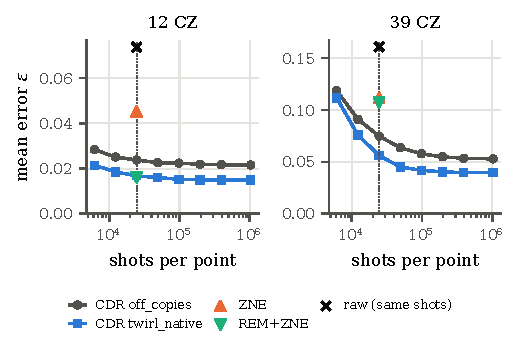
\includegraphics[width=\columnwidth]{figs/fig_cost_curve.pdf}
\caption{Equal-budget re-analysis (night A, exploratory): expected CDR error vs.\ shots per
point, from subsampling the archived counts (200 draws per point; the rightmost point is the
measured design). ZNE, REM+ZNE and raw are single measurements at 24,576 shots (dotted
line).}
\label{fig:cost}
\end{figure}

\subsection{ZNE needs readout correction; CDR does not}
At 12~CZ the signed ZNE error is positive at all 8 points ($+0.0095$ to $+0.0765$, mean
$\approx+0.045$): a $\lambda$-independent offset that Richardson passes through
(Section~\ref{sec:background}). REM lowers the ZNE error from 0.045 to 0.016, at 8/8 points
(ratio 0.29 [0.19, 0.42], $p=0.008$\expl); the remaining offset of about $+0.016$ is consistent
with $T_1$ relaxation before readout. Without REM, ZNE does not beat raw at 12~CZ ($p=0.47$,
pre-registered H4 fails); with REM it beats uncorrected raw in 6/8 points ($p=0.078$\expl) and
REM-corrected raw in 4/8 ($p=0.31$\expl). CDR is invariant to REM (0.0216$\to$0.0211,
0.0529$\to$0.0528), because its intercept absorbs the offset. At 39~CZ, REM barely changes ZNE
(0.112$\to$0.107): the error there is collapse, not readout. A ZNE--CDR comparison without REM
is therefore not a comparison of extrapolation and regression.

\subsection{ZNE collapse: which diagnostics see it}
At 39~CZ ZNE beats raw at 8/8 points ($p=0.004$), but garbage folding, which cannot
extrapolate anything, does as well (0.103; genuine below garbage in 2/8, $p=0.84$); at
12~CZ genuine beats garbage (0.045 vs.\ 0.137, 7/8, $p=0.012$). At 39~CZ, $E(\lambda=5)$
differs from the mean garbage floor by $-0.002$ to $+0.006$ at every point while the ideal
values span $-0.43$ to $+0.17$ (Fig.~\ref{fig:zne}, right): the extrapolation is the rescaling
$\tfrac{15}{8}E_1-\tfrac78f$, a replication of~\cite{koster2026}. The pre-registered diagnostics
passed this rung: median $W_{\text{neg}}=0$ and median SNR against zero 4.1 ($\ge2$). The
floor-referenced SNR detects it (median 0.8 against the point's own garbage floor, 0.4 against
the mean floor; 11.8 at 12~CZ), as does the floor-tracking distance (median 0.016 at 39~CZ vs.\
0.172 at 12~CZ, where, however, garbage at $\lambda=5$ is not yet at the floor, so the 12-CZ
value partly reflects the choice of $f$). No SNR variant predicted the per-point ZNE gain
(Spearman $|\rho|\le0.05$\expl). Exponential extrapolation with a measured floor is undefined at
5 of 8 points at 39~CZ. The same circuit measured in the ZNE and in the CDR block differs more
than shot noise at 39~CZ ($\chi^2/\mathrm{df}=2.4$ vs.\ 1.0 at 12~CZ\expl), a direct sign of
block-to-block drift.

\begin{figure}[t]
\centering
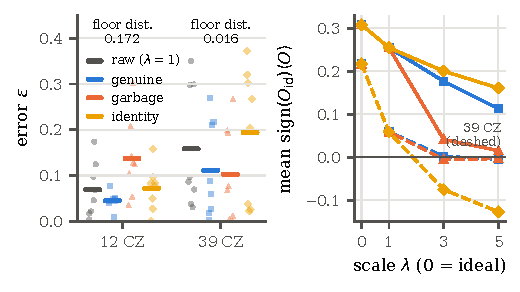
\includegraphics[width=\columnwidth]{figs/fig_zne_window.pdf}
\caption{ZNE in night A. Left: per-point errors (dots) and means (bars) of raw ($\lambda=1$),
genuine, garbage and identity folding; annotation: median floor-tracking distance. Right: mean
of $\mathrm{sign}(\Oid)\ev{O}(\lambda)$ with the ideal at $\lambda=0$ (solid 12~CZ, dashed
39~CZ). At 39~CZ genuine and garbage coincide at the floor for $\lambda\ge3$; identity folding
drifts towards $+1$.}
\label{fig:zne}
\end{figure}

\subsection{The identity-folding control is invalid on hardware}\label{sec:identity}
Identity folding has the CZ and PRX counts and ASAP duration of genuine folding and returns the
ideal value in noiseless simulation (both checked on the archived circuits), yet on ODRA its
$\ev{O}$ drifts towards $+1$: $+0.16$ / $+0.28$ at $\lambda=3,5$ for 12~CZ and $+0.40$ / $+0.57$
for 39~CZ. A device-model simulation with the night's calibration ($T_1=13$--24\,\textmu s)
reproduces the direction and growth ($+0.06$ / $+0.13$ and $+0.28$ / $+0.44$), and the drift
vanishes when $T_1\to\infty$ (within $\pm0.03$) but not when $T_2$ or dynamical decoupling is
changed. Half of the identity block is a bare CZ sequence and the other half gate--inverse
pairs, so the state after $U$ is never ``processed'' again and amplitude damping pushes it to
$\ket{00000}$, whereas in $U(U^\dagger U)^k$ relaxation happens mid-circuit and is rotated by
the final $U$. A gate-count-matched control is not a noise-matched control; it should be
validated in a device model before use. We draw no conclusion from it.

\subsection{Twirling: fit linearity, frame variance and the log floor}
At equal budget, native twirling lowered the mean CDR error from 0.053 to 0.040 at 39~CZ (7/8
pairs, ratio 0.68 [0.48, 1.08]) and from 0.022 to 0.015 at 12~CZ (4/8, ratio 1.41)
(Fig.~\ref{fig:twirl}). The pre-registered H1 on the 16 available pairs is not supported
($p=0.35$, ratio 0.98). The 12-CZ ratio above 1 is an artefact of the log floor: two
\arm{off\_copies} errors of $6\times10^{-4}$ and $5.5\times10^{-5}$ (the latter at the
$10^{-4}$ floor) drive it, and the ratio becomes 0.99 / 0.84 / 0.85 for floors of $10^{-3}$ /
$3\times10^{-3}$ / $10^{-2}$; the arithmetic and RMS ratios are 0.69 and 0.60. It is not shot
noise either: the \arm{off\_copies} error (0.022) is about ten times its shot-noise
contribution (0.002). The twirl~$\times$~rung interaction (ratio of ratios 0.48 [t-CI 0.15,
1.52], $p=0.20$\expl) is not established.

Two observations are consistent across rungs\expl. (i) Twirling raises the CDR fit's $r^2$:
mean 0.972$\to$0.989 at 12~CZ (7/8 points) and 0.789$\to$0.905 at 39~CZ (8/8), while it
leaves the raw target error unchanged; a single noise model fitted to all training circuits of
the window also fits twirled data better (RMSE 0.023$\to$0.013). (ii) Native frames are noisy:
the frame-to-frame variance of a circuit's $\ev{O}$ is 29 times the shot variance at 12~CZ (SD
0.027) and 12 times at 39~CZ (SD 0.018), whereas copies show none (ratio 0.8). With $M=6$
frames this variance makes up about 55\% (12~CZ) and 25\% (39~CZ) of the twirled CDR's squared
error; removing it, the estimated RMS bias is 0.013 vs.\ 0.032 (twirled vs.\ untwirled) at
12~CZ and 0.043 vs.\ 0.067 at 39~CZ. The binding resource of native twirling here is the
number of frames, not shots per frame. Twirling helps empirically, but the mechanism goes
beyond a simple coherent $ZZ$ error on the CZ; we do not identify it. Logical vs.\ native
twirling (H3, $p=0.85$) is not interpretable: on the \arm{shared\_random} set all points share
their training circuits, so the 16 pairs are not independent. \arm{spread} (H6, $p=0.55$) was
worse than \arm{twirl\_native} at 39~CZ (0.068 vs.\ 0.040).

\begin{figure}[t]
\centering
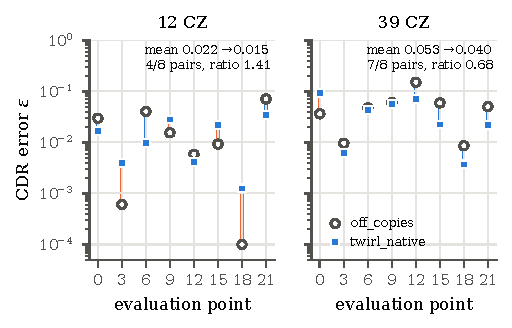
\includegraphics[width=\columnwidth]{figs/fig_twirl_pairs.pdf}
\caption{Per-point CDR error of \arm{off\_copies} (circles) and \arm{twirl\_native} (squares)
at equal budget, night A; blue: twirling better, orange: worse; ratio: geometric mean with the
pre-registered $10^{-4}$ floor, which drives the 12-CZ value (see text).}
\label{fig:twirl}
\end{figure}

\subsection{Noise-axis decomposition: duration vs.\ CZ count (P5)}
Table~\ref{tab:p5} and Fig.~\ref{fig:p5} give the identity-insertion results. At fixed gates,
each microsecond raises the raw error by a factor 1.43 (CI 1.27--1.61); this survives the
small-cluster corrections ($p=1.7\times10^{-4}$ with $t(7)$, $p=0.008$ with the wild
bootstrap, which is its resolution limit) and is the one confirmed pre-registered hypothesis
(H7b; Holm-adjusted wild-bootstrap $p\approx0.04$). At fixed duration, CZ pairs do not change
the log raw error on average (0.96 per 10~CZ, $p=0.69$), but this is not evidence of absence:
mean raw errors of CZ pairs exceed their idle twins at all three levels (0.094 vs.\ 0.090,
0.159 vs.\ 0.112, 0.177 vs.\ 0.147); dropping the two points with $|\Oid|<0.1$, where the error is
an offset rather than a contraction, gives 1.11 per 10~CZ ($p=0.008$, $t(5)$\expl); and the
CZ-vs-idle contrast is fully confounded with block time and partly with the calibration
change (Section~\ref{sec:methods}). H7a is therefore \emph{unresolved}. After CDR the picture
reverses: the residual grows with CZ count (1.34 per 10~CZ, $p=0.018$ with $t(7)$, 0.016 wild
bootstrap) and not significantly with duration. Idle insertion barely affects the CDR error
(0.021 base; 0.014 / 0.031 / 0.037 with idle) while CZ pairs raise it (0.022 / 0.072 / 0.074),
and $r^2$ drops at 36 and 52~CZ (median 0.81 and 0.67 vs.\ 0.94 and 0.87 for the idle twins):
time-driven contraction is shared by training and target circuits, which is what CDR's affine
map learns, while the CZ-driven part transfers worse from Clifford circuits. Dropping
\texttt{star\_cz52} (calibration changed) or both \texttt{star\_cz24} and \texttt{star\_cz52}
leaves the conclusions unchanged (raw $\times1.48$ per \textmu s, $p\le0.002$; raw $\times1.03$
per 10~CZ, $p\ge0.87$; after CDR $\times1.59$ and $\times1.70$ per 10~CZ, $p\le0.006$; all $t(7)$).

\begin{table}[t]
\caption{P5 regression (56 observations, 8 points, point fixed effects). CI and first $p$:
cluster-robust with $t(7)$; second $p$: exact wild-cluster bootstrap.}
\label{tab:p5}
\centering\footnotesize
\setlength{\tabcolsep}{4pt}
\begin{tabular}{@{}llcccc@{}}
\toprule
outcome & term & factor & 95\% CI & $p_{t(7)}$ & $p_{\text{wild}}$ \\
\midrule
raw & +10 CZ (fixed time) & 0.96 & 0.74--1.24 & 0.69 & 0.68 \\
raw & +1\,\textmu s (fixed gates) & 1.43 & 1.27--1.61 & $1.7\!\times\!10^{-4}$ & 0.008 \\
after CDR & +10 CZ & 1.34 & 1.07--1.67 & 0.018 & 0.016 \\
after CDR & +1\,\textmu s & 1.32 & 0.69--2.53 & 0.35 & 0.31 \\
\bottomrule
\end{tabular}
\end{table}

\begin{figure*}[t]
\centering
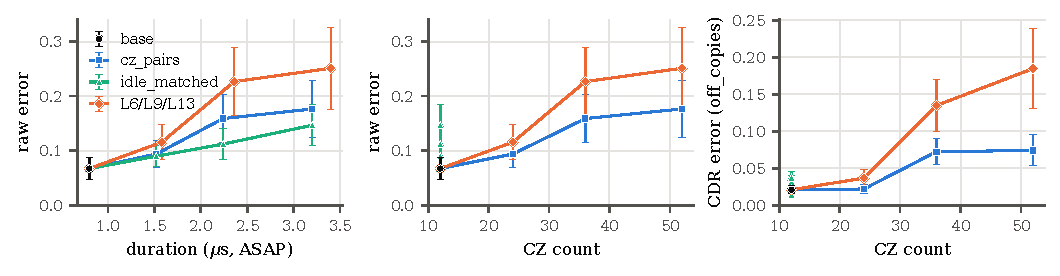
\includegraphics[width=\textwidth]{figs/fig_p5_depth.pdf}
\caption{Identity insertion (night P5, \arm{off\_copies}; mean $\pm$ SE over 8 points). Left:
raw error vs.\ ASAP duration; centre: raw error vs.\ CZ count; right: CDR error vs.\ CZ count.
The $L$=6/9/13 classifiers are different functions and are shown for reference only. Idle and
CZ-pair blocks ran at different times of the night (Section~\ref{sec:methods}).}
\label{fig:p5}
\end{figure*}

\subsection{Negative results}
Table~\ref{tab:neg} collects methods that did not beat plain CDR at equal budget. Most
instructive is noise-model-informed CDR: a single low-parameter noise model per window
($E=f+g\,e^{-a_{\text{cz}}n_{\text{CZ}}-a_tT-a_pn_{\text{PRX}}/10}\Oid$), fitted to all
training circuits, misfits them by 0.023 (night A, untwirled), 0.013 (twirled) and 0.043 (P5)
against a shot noise of about 0.002, and as a mitigator is worse than CDR in 8 of 9 rung--arm
cells; cross-validated shrinkage towards it selects no shrinkage. Different evaluation points
have different noise responses, which per-point CDR captures and a shared model does not.
Composing ZNE with CDR double-corrects the same attenuation (CDR slope 1.22 / 2.50 vs.\ ZNE's
implied gain 1.18 / 1.34). On P5, the pre-specified vnCDR variant failed; of $\sim$18
secondary variants one (idle axis, 6 inserted delays) looked strong (ratio 0.57, 7/8), but the
same method with 12 or 20 delays was worse---a forking-paths pattern that motivated the interleaved,
pre-registered \texttt{w02vn}.

\begin{table}[t]
\caption{Negative results (exploratory, equal budget unless noted; ratio = geometric mean
vs.\ plain CDR, $>1$ worse).}
\label{tab:neg}
\centering\footnotesize
\setlength{\tabcolsep}{3pt}
\begin{tabular}{@{}L{0.42\columnwidth}L{0.54\columnwidth}@{}}
\toprule
method & result \\
\midrule
noise-model CDR, one model per window & A: ratio 1.65 [0.61, 4.37] (untw.), 2.10 [1.22, 3.67] (tw.); P5: 4.11 [2.58, 6.60], 7/40 wins \\
$a\cdot$ZNE$+b$ (CDR map on ZNE) & 0.066 vs.\ 0.022 (12~CZ, 2/8); 0.107 vs.\ 0.053 (39~CZ) \\
(CDR+ZNE)/2; inverse-variance mix & between CDR and ZNE \\
leave-one-out stacking of CDR, ZNE & ties CDR (4/8, 3/8 wins) \\
CDR + duration (or PRX) covariate & 0.054 vs.\ 0.022, 1/8 wins (12~CZ) \\
attenuation-transfer correction & changes errors by $\le0.001$ \\
vnCDR on P5 (pre-specified: 12 pairs, 2 axes, intercept; levels from separate blocks) & ratio 1.12 [0.69, 1.73], 2/8, $p=0.73$ (one-sided) \\
\arm{spread} (120 circuits $\times$ 1 frame), H6 & $p=0.55$; worse at 39~CZ (0.068 vs.\ 0.040) \\
identity-folding ZNE control & invalid ($T_1$), Sec.~\ref{sec:identity} \\
\bottomrule
\end{tabular}
\end{table}

\subsection{Interleaved two-axis vnCDR (\texttt{w02vn})}\label{sec:w02vn}
Status: \TBD{run date, number of circuits completed, interruptions}. Calibration: \TBD{calibration
set IDs; blocks with a change}. Complete points: \TBD{n of 8; excluded points}. Primary test
(two-axis vnCDR vs.\ CDR, equal budget of 4.1\,M shots per point): mean error \TBD{vnCDR vs.\
CDR}, geometric-mean ratio \TBD{ratio [95\% CI]}, wins \TBD{wins/8}, one-sided Wilcoxon
\TBD{p}; verdict: \TBD{SUCCESS / NOT SUPPORTED}. Sensitivity without calibration-change blocks:
\TBD{ratio, p}. Secondary (no claims): \TBD{one-axis vnCDR (time, CZ), no-intercept, $3\times$
budget, raw vs.\ CDR}. Comparison with the simulated prediction: \TBD{hardware CDR error vs.\
simulated 0.0065 at 4.1\,M}.

\subsection{Pilot measurements (exploratory)}
In pilot windows on the 12-CZ circuit, the ZNE variance constant was measured as
$\kappa=15.8\pm1.7$ (uniform $\{1,3,5\}$, predicted 14.66), $12.5\pm1.1$ and $20.7\pm14.7$ in two
Neyman windows (predicted 11.6 and 11.9), and $26.0\pm3.3$ and $25.7\pm11.3$ for Neyman
$\{1,3,5,7\}$ (predicted 36.7 and 37.2); an archival uniform $\{1,3,5,7\}$ run gave $48\pm6$
(predicted 44.6). The uncertainties are within-window; the spread between windows shows the
real uncertainty is larger. Pilot twirling ratios at 12~CZ (0.22--0.57) were far below
\texttt{w01}'s, a winner's-curse pattern that a pre-analysis plan built on pilots does not
prevent. Decision changes of the classifier occur only where $|\hat O-E|\ge|E|$, i.e.\
mechanically at small margins; in night A one of 16 decisions changed (margin 0.028).

% ---------------------------------------------------------------------------------------
\section{Discussion}\label{sec:discussion}

\emph{What the protocol bought.} Without its controls, this dataset would have supported a
``regime map'': ZNE for shallow circuits, ZNE still useful at 39~CZ, CDR best everywhere,
twirling hurting at 12~CZ and halving the error in pilots. Each element dissolves under one
control (Table~\ref{tab:pitfalls}): the equal-budget re-analysis and REM remove CDR's advantage
at 12~CZ; the garbage control and a floor-referenced SNR expose the 39-CZ ZNE gain as collapse;
the floor sensitivity removes the twirling penalty; the confirmatory test does not support
H1. What stands is narrower and, we think, more useful: CDR at modest budgets is a robust
mitigator on this device; ZNE needs REM and an independent collapse check; twirling improves
CDR's linearity but needs many more frames than the usual handful; and decoherence during the
schedule, not CZ count, dominates the raw error at fixed gates, while the CZ-driven error is
what CDR fails to remove. The last point suggests noise scaling along two axes, which is what
\texttt{w02vn} tests under conditions designed to give it a fair chance: interleaved levels,
the rung where simulation predicts a gain, and four times the budget.

\begin{table}[t]
\caption{Pitfalls confirmed on ODRA~5 and the control that exposed each.}
\label{tab:pitfalls}
\centering\footnotesize
\setlength{\tabcolsep}{3pt}
\begin{tabular}{@{}L{0.29\columnwidth}L{0.36\columnwidth}L{0.29\columnwidth}@{}}
\toprule
pitfall & evidence & remedy \\
\midrule
unequal budgets & CDR $42\times$ ZNE; CDR saturates at $4$--$8\times$ & cost curves from counts; \arm{off\_copies} \\
offset passes Richardson & ZNE $0.045\to0.016$ with REM & REM or intercept \\
collapse looks like gain & garbage $\approx$ genuine at 39~CZ & garbage control; SNR vs.\ floor \\
blind diagnostics & $W_{\text{neg}}=0$, SNR$_0=4.1$ & do not use alone \\
count-matched $\neq$ noise-matched & identity drifts to $+1$ ($T_1$) & validate in device model \\
log floor $\ll$ shot SE & twirl ratio 1.41$\to$0.99 & floor at shot SE; RMS too \\
too few frames & frame var.\ 12--29$\times$ shot & more frames, fewer shots \\
unseeded routing & 0--2/10 skeleton matches & one path; native training \\
unmerged frames & 40$\to$92 1q gates & merge after twirling \\
block confounds & idle/CZ blocks hours apart; cal.\ change & interleave within jobs \\
8 clusters & $p$: $5\!\times\!10^{-13}\to0.008$ & $t(G-1)$, wild bootstrap \\
shared training set & H3 pairs dependent & per-point seeds \\
pilot-based hypotheses & 12-CZ ratios 0.22--0.57 vs.\ 1.41 & confirmatory window \\
\bottomrule
\end{tabular}
\end{table}

\emph{Deviations from pre-registration (\texttt{w01}).} (i) The plan was frozen after night A
had begun, and the first part of night A ran on an earlier commit with a non-clean tree
(resumed on the pre-registration commit); an independent audit recomputed every number from the
archived circuits and counts, but whether the circuits run under the earlier commit match the
frozen code has not been verified.
(ii) Night B was not completed, so H1, H3 and H6 were tested on 16 instead of 32 pairs; the
frozen code ran on the incomplete data without a warning. (iii) The plan states H7a/H7b as
two-sided, the frozen code tests them one-sided; we report the two-sided values
(Table~\ref{tab:p5}), which do not change the decisions. (iv) The pre-registered cluster-robust
normal reference with 8 clusters is anti-conservative; we add $t(7)$ and wild-bootstrap
$p$-values. (v) The pre-registered H4 SNR criterion is referenced to zero; we reinterpret it
against the floor post hoc and report both. (vi) The log floor of $10^{-4}$ is retained for
the registered tests; higher floors are sensitivity analyses. (vii) All REM, equal-budget,
$r^2$, frame-variance, hybrid and noise-model analyses were not pre-registered. For
\texttt{w02vn}: \TBD{deviations, if any}.

\emph{Limitations.} One device and one window: no between-window variance, and night A and the
analysed P5 rungs share one calibration set. Eight points per rung make per-rung tests weak.
Each condition is a single block, so arm contrasts are arm~$\times$~time contrasts; within-block
copies show no excess variance, but between blocks we see drift at 39~CZ. The two rungs are
different classifiers, and the mean-$Z$ observable has a non-zero floor and Clifford training
values that are often zero; other observables change both. Durations are computed, not
measured. The device model reproduces only part of the hardware error (CDR three times lower in
simulation). Some bibliographic details of 2026 preprints are not yet verified.

% ---------------------------------------------------------------------------------------
\section{Conclusion}
On a five-qubit star processor, an evaluation protocol with equal-budget controls,
matched-cost negative controls, pre-registration and full provenance turned most apparent QEM
effects into identifiable pitfalls: budget mismatch, readout offsets passed by Richardson,
undetected ZNE collapse, a control that matched gate counts but not noise, a log-floor
artefact, frame-count-limited twirling and block confounds. The robust physical finding is a
decomposition of the noise axis: duration drives the raw error at fixed gates, and the error
that survives CDR is the CZ-driven part. Whether scaling both axes inside CDR pays on hardware
is the subject of the pre-registered \texttt{w02vn} test: \TBD{one-sentence w02vn conclusion}.

\section*{Data and code availability}
Raw counts, manifests, derived tables, frozen models, both pre-registrations (tags
\texttt{prereg-v1}, \texttt{prereg-vn1}), the offline re-analysis and figure scripts will be
made available at \TBD{repository URL / DOI}.

\section*{Acknowledgment}
\TBD{acknowledgments: access to ODRA~5, KN Axion, funding}.

\bibliographystyle{IEEEtran}
\bibliography{refs}

\end{document}
